%! suppress = MissingImport
\subsection{Seven-Segment Display Module}

Examine the 7-segment display module.
Notice that the header has five pins (Figure~\ref{fig:display-module-header}): \texttt{VCC} (common collector voltage), \texttt{GND} (ground), \texttt{DIN} (data in), \texttt{CS} (chip select), and \texttt{CLK} (clock).
When the display module is oriented for viewing, these header pins will be on the left.

Figure~\ref{fig:display-diagram} shows a diagram of the wiring to connect the display module to the breadboard.

\begin{figure}
    \centering
    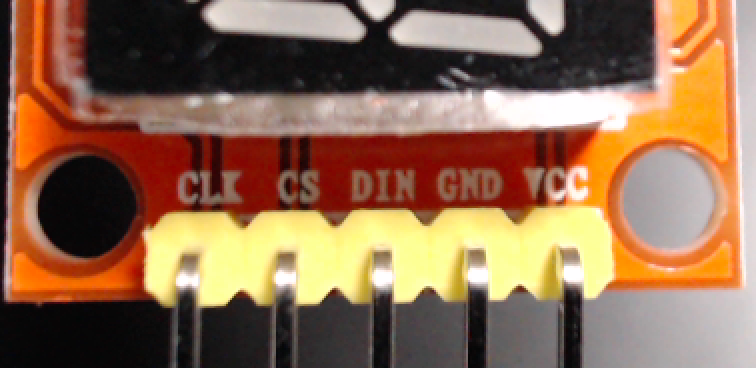
\includegraphics[width=5cm]{display/display-module-header}
    \caption{The display module's header has five pins.
    \label{fig:display-module-header}}
\end{figure}

\begin{figure}
    \centering
    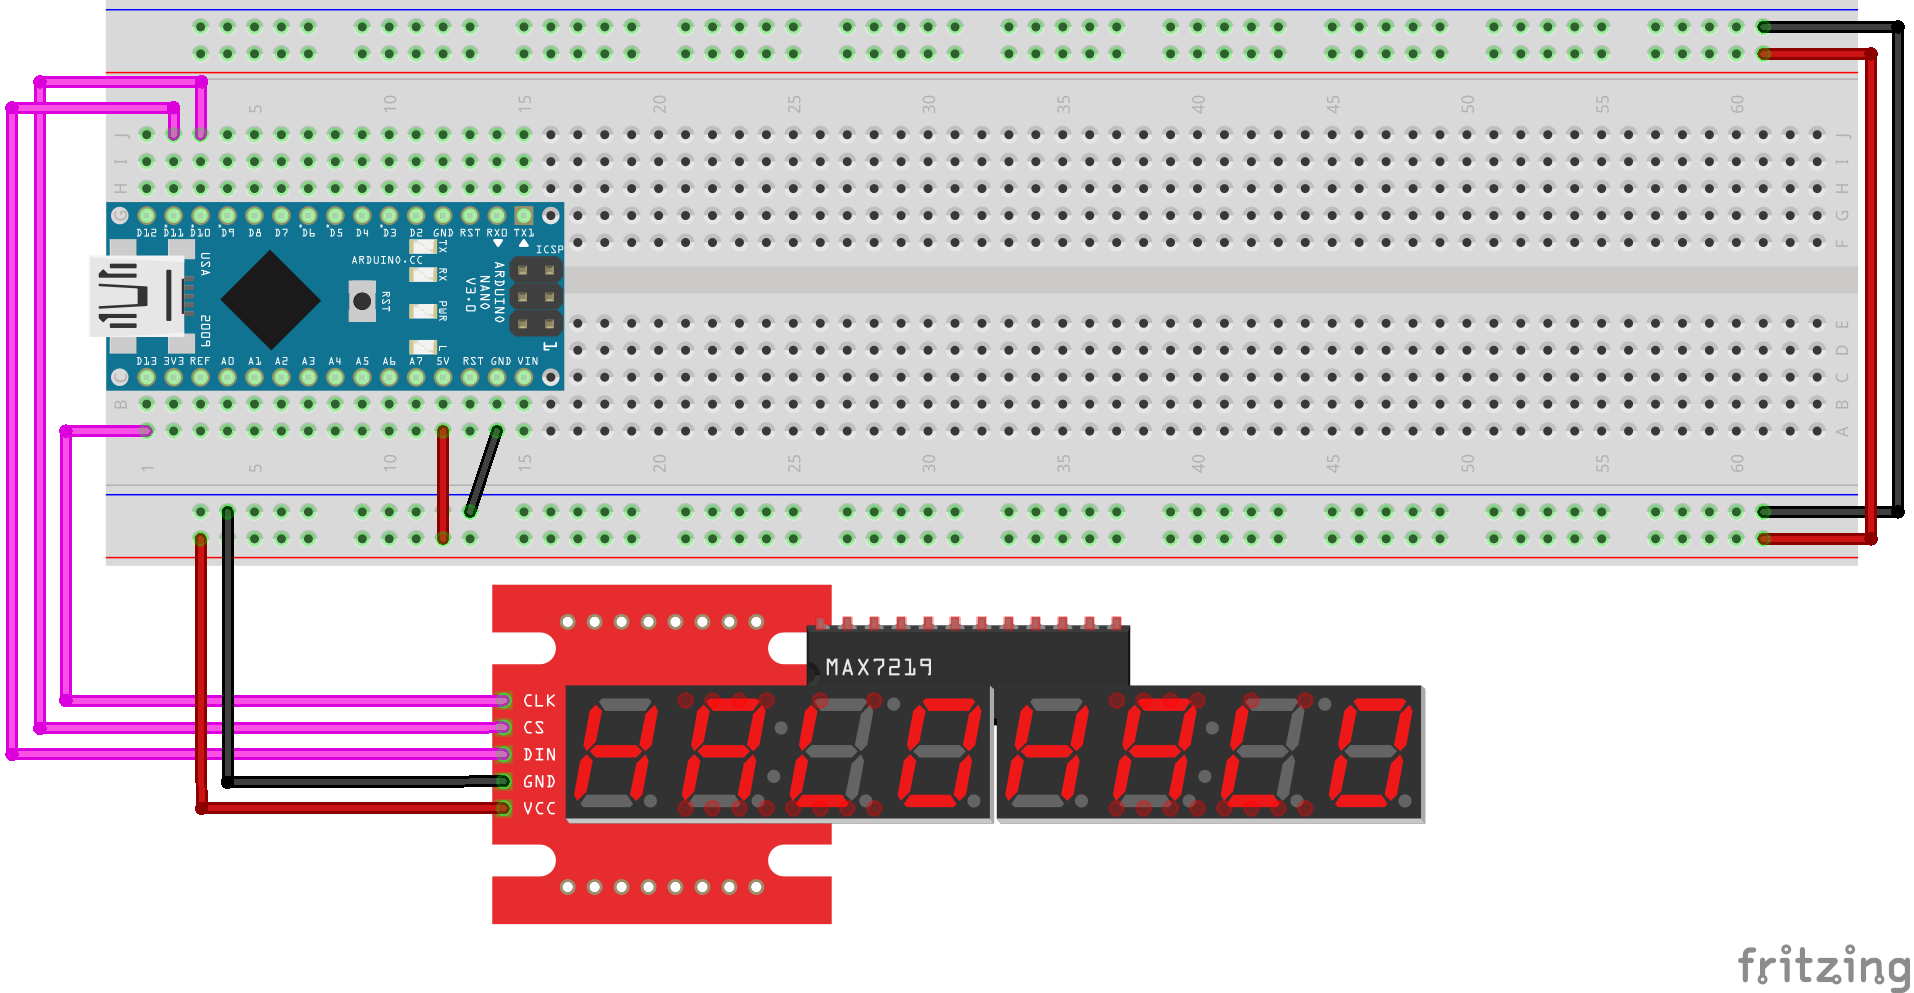
\includegraphics[width=0.9\textwidth]{fritzing_diagrams/display-max7219}
    \caption{Diagram of display module's connections to the breadboard.
    \label{fig:display-diagram}}
\end{figure}

\disconnect\

Take the 5-conductor female-to-male rainbow cable and attach the five female connectors to the display module's five header pins;
see Figure~\ref{fig:display-module-female-connectors}.

As you insert the male connectors into the breadboard, you may have to partially separate the wires at the male end.
In the interest of keeping track of which wires are used for which purposes, do not fully separate the wires.
Identify the wire that is connected to the display module's \texttt{CLK} pin;
insert the male end of this wire in contact point a1 (electrically connected to the \developmentboard's \texttt{D13} pin in c1); see Figure~\ref{fig:display-module-CLK}.
Insert the male end of the \texttt{CS} wire into contact point j3 (electrically connected to the \developmentboard's \texttt{D10} pin in g3); see Figure~\ref{fig:display-module-CS}.
Insert the male end of the \texttt{DIN} wire into contact point j2 (electrically connected to the \developmentboard's \texttt{D11} pin in g2); see Figure~\ref{fig:display-module-DIN}.
Insert the \texttt{GND} wire into a \ground, and the \texttt{VCC} wire into a \power\ (Figure~\ref{fig:display-module-power}).

\begin{figure}
    \centering
    \subfloat[Connect the female ends of the 5-conductor cable to the display module's header pins (your colors may be different).] {
        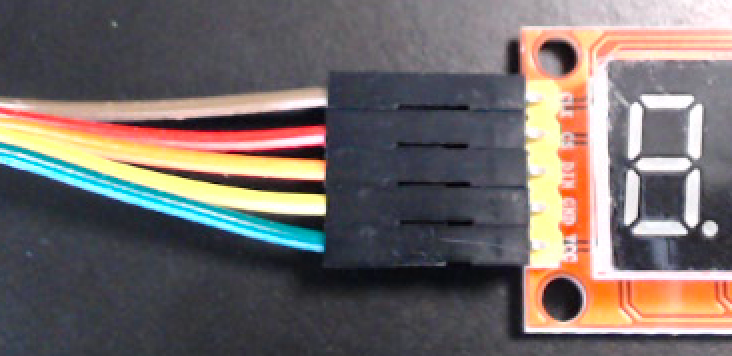
\includegraphics[width=0.27\textwidth]{display/display-module-female-connectors}
        \label{fig:display-module-female-connectors}
    }
    \hfil
    \subfloat[The display module's clock will be driven by \texttt{D13}.] {
        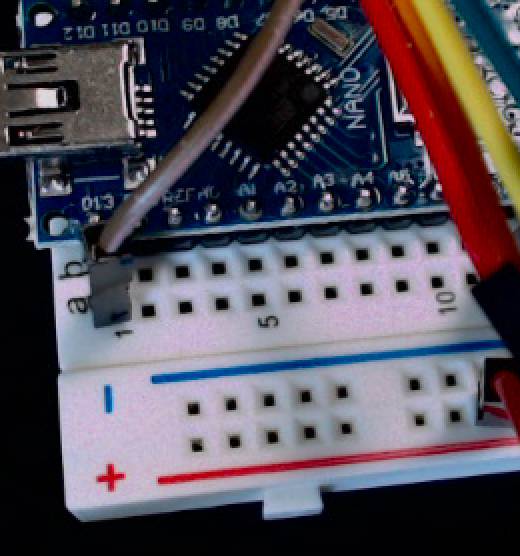
\includegraphics[width=0.27\textwidth]{display/display-module-CLK}
        \label{fig:display-module-CLK}
    }
    \hfil
    \subfloat[The display module's chip-select will be driven by
    \texttt{D10}.] {
        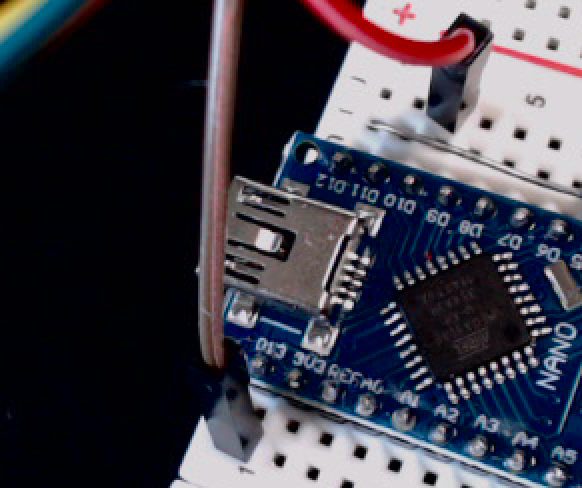
\includegraphics[width=0.27\textwidth]{display/display-module-CS}
        \label{fig:display-module-CS}
    }

    \subfloat[The display module's data-in will be driven by \texttt{D11}] {
        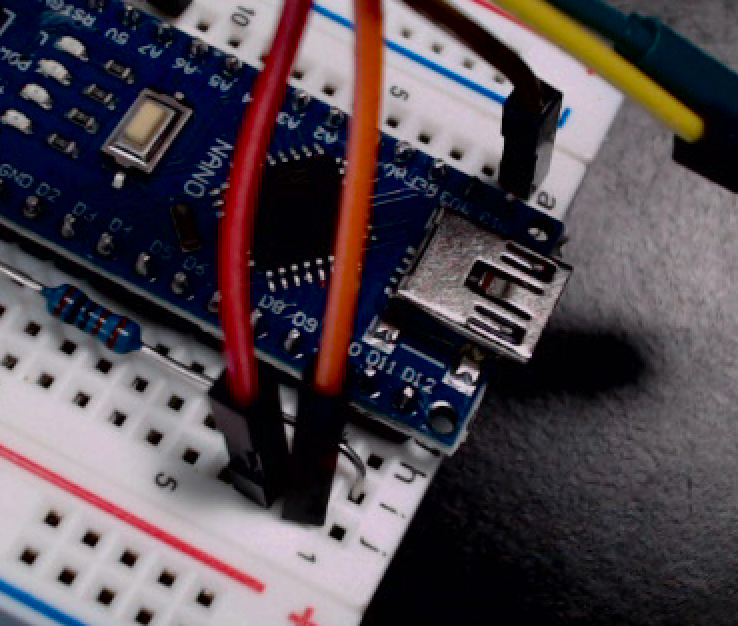
\includegraphics[width=0.27\textwidth]{display/display-module-DIN}
        \label{fig:display-module-DIN}
    }
    \hfil
    \subfloat[The display module will be powered by the breadboard's power bus] {
        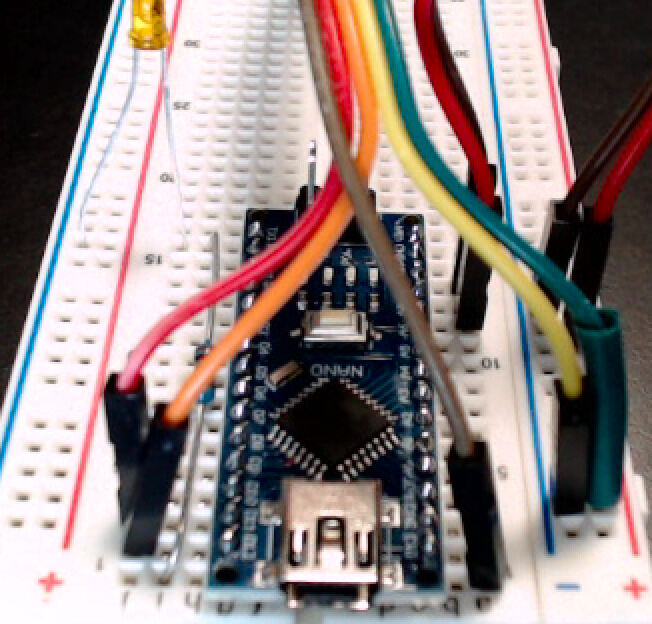
\includegraphics[width=0.27\textwidth]{display/display-module-power}
        \label{fig:display-module-power}
    }
    \caption{Connecting the Display Module.}
\end{figure}

When you have finished connecting the display module, there should be the electrical connections described in Table~\ref{tab:display}.

\begin{table}
    \begin{center}\begin{tabular}{||c|c|c||} \hline\hline
    Display Module Pin  & \developmentboard\ pin    & Pulled High/Low \\ \hline
    \texttt{CLK}         & \texttt{D13}  & \\
    \texttt{CS}          & \texttt{D10}  & \\
    \texttt{DIN}         & \texttt{D11}  & \\
    \texttt{GND}         &               & Pulled Low \\
    \texttt{VCC}         &               & Pulled High \\ \hline\hline
    \end{tabular}\end{center}
    \caption{Electrical Connections for External LED.\label{tab:display}}
\end{table}

\checkpoint{connected the display module to the breadboard}

In the Arduino IDE, open \textit{DisplayTest.ino}.
Connect your \developmentboard\ to the computer.
Compile \textit{DisplayTest.ino} and upload it to your \developmentboard.
You should see {\dviiseg 8.} move back and forth across the display (Figure~\ref{fig:display-test}).
You may be able to see the \developmentboard's built-in LED blink rapidly: recall that it's connected to pin 13, which is used as the clock signal when the \developmentboard\ sends data to the display module.

\begin{figure}
    \centering
    \animategraphics[autoplay,palindrome,height=5cm]{10}{display/animations/displaytest-}{0}{7}
    \caption{\textit{DisplayTest.ino} illuminates all segments on a digit, one digit at a time. \label{fig:display-test}}
\end{figure}
